\section{Orthonormal Bases}\label{sec: orth}

In this section, we discuss the conditions on $m-$ functions such that the corresponding MRA forms an orthonormal bases. 
%consider orthonormal bases with $m-$functions defined in \eqref{eq: m0} and \eqref{eq: mj} whose supports mainly corresponding to the partition of $S_0$ in Fig.\ref{fig: partition}.
%we always consider a multi-resolution system with scaling function $\phi$ and quasi-shearlets $\psi^j$, {\small$ j = 1,\dots,6$} defined by $(M_0, D_2)$ and $(M_j, Q)$, {\small$j = 1,\dots,6$} respectively. Furthermore, the essential support of $M_j$'s corresponds to the partition of $\mathbf{S}_0$ in a shearlet system.

%The construction of \eqref{eq: MRA} reduces to design $m_0$ in \eqref{eq: m0} and $m_j, j= 1,\cdots,6$ in \eqref{eq: mj}.
We begin with the two key conditions, i.e. {\it identity summation} and {\it shift cancellation}, on $m-$functions such that the system \eqref{eq: MRA} is perfect reconstruction (PR) or equivalently a Parseval frame in MRA.% weaker than the orthonormal condition.

%\subsection{Identity summation and shift cancellation}
\subsection{orthonormal conditions on $m-$functions}
In MRA, \eqref{eq: MRA} is PR if $\forall f\in L_2(\mathbb{R}^2)$,
\begin{equation}
\textstyle \sum_k\langle f,\phi_{0,k}\rangle\phi_{0,k} = \sum_k\langle f,\phi_{1,k}\rangle\phi_{1,k} + \sum_j\sum_k\langle f,\psi^{j}_{1,k}\rangle\psi^j_{1,k}.\label{eq: PR}
\end{equation}
Using \eqref{eq: m0} and \eqref{eq: mj} together with the admissibility of the frequency partition, this condition on $\phi$ and $\psi^j$'s yields:
\begin{thm}\label{thm: conds}
The perfect reconstruction condition holds for \eqref{eq: MRA} iff the following two conditions hold
\begin{align}\label{eq: id-sum}
|m_0(\boldsymbol{\omega})|^2 + \sum_{j = 1}^6|m_j(\boldsymbol{\omega})|^2 = 1
\end{align}
\begin{equation}\label{eq: shift-cancel}
 \begin{cases}
%M_0(\boldsymbol{omega})\overline{M_0(\boldsymbol{omega}+\boldsymbol{\gamma})} + 
\sum_{j = 0}^6m_j(\boldsymbol{\omega})\overline{m_j(\boldsymbol{\omega} + \boldsymbol{\pi})} = 0, & \boldsymbol{\pi}\in \Gamma_0\setminus\{\boldsymbol{0}\}\\[.5em]
\sum_{j=1}^6m_j(\boldsymbol{\omega})\overline{m_j(\boldsymbol{\omega}+\boldsymbol{\pi})} = 0, & \boldsymbol{\pi}\in\Gamma_1\setminus\Gamma_0
\end{cases}
\end{equation}
%where  $\Lambda = (QD\mathbb{Z}^2)^*/(\mathbb{Z}^2)^*,\,\Gamma = (D\mathbb{Z}^2)^*/(\mathbb{Z}^2)^*.$ %$\{(\frac{\pi}{2},\frac{\pi}{2}),(\frac{3\pi}{2},\frac{\pi}{2}),(\frac{\pi}{2},\frac{3\pi}{2}),(\frac{3\pi}{2},\frac{3\pi}{2}),$ $(0,0),(0,\pi),(\pi,0),(\pi,\pi)\}$
\end{thm}

Theorem \ref{thm: conds} is a corollary of Prop. 1 and Prop. 2 in \cite{durand2007}. We give an alternate proof in Appendix \ref{app: cond-thm}.
In Theorem \ref{thm: conds}, Eq. \eqref{eq: id-sum} is the {\it identity summation} condition, guaranteeing conservation of $l_2$ energy; Eq. \eqref{eq: shift-cancel} is the {\it shift cancellation} condition such that aliasing is canceled correctly in reconstruction. %, such that downsampling of scaling and shearlet coefficients is valid. 
 %$\Lambda = \{(\frac{\pi}{2},\frac{\pi}{2}),(\frac{3\pi}{2},\frac{\pi}{2}),(\frac{\pi}{2},\frac{3\pi}{2}),(\frac{3\pi}{2},\frac{3\pi}{2}),$ $(0,0),(0,\pi),(\pi,0),(\pi,\pi)\},\Gamma = \{(0,0),(0,\pi),(\pi,0),(\pi,\pi)\}$ are the sets of shifts associated to quincunx-dyadic dilation $QD$ and dyadic dilation $D$ respectively.
%Each $M_j$ contributes a term $M_j(\boldsymbol{omega})\overline{M_j(\boldsymbol{omega} + \boldsymbol{\nu})}$ in the cancellation condition of any shift $\boldsymbol{\nu}$ corresponding to the downsampling scheme of $M_j$.

%\subsection{Extra condition for basis}
%By Theorem \ref{thm: conds}, the system \eqref{eq: MRA} is a Parseval frame ; 
For  \eqref{eq: MRA} to be an orthonormal basis,  $\{\phi_{\boldsymbol{k}}\}_{\boldsymbol{k}\in\mathbb{Z}^2}$ need to be an orthonormal basis, which is determined by $m_0$ in \eqref{eq: phi-m0}. In 1D MRA, Cohen's theorem in \cite{cohen1992biorthogonal} provides a necessary and sufficient condition on $m_0$ such that \eqref{eq: MRA} is an orthonormal basis. %Such a condition in 1D wavelet MRA is given by Cohen \cite{cohen1992biorthogonal}. 
We generalized this theorem to 2D in \cite{yin2014orthshear}.
\begin{thm}\label{thm: basis cond}
Assume that $m_0$ is a trigonometric polynomial with $m_0(0)=1$, and define $\hat{\phi}(\boldsymbol{\omega})$ as in \eqref{eq: phi-m0}.\\
If $\phi(\cdot - \boldsymbol{k}),\boldsymbol{k}\in\mathbb{Z}^2$ are orthonormal, then $\exists K$ containing a neighborhood of 0, s.t. $\forall\boldsymbol{\omega}\in S_0,\,\boldsymbol{\omega}+2\pi\mathbf{n}\in K$ for some $\mathbf{n}\in\mathbb{Z}^2, $ and $\inf_{k>0,\,\boldsymbol{\omega}\in K}|m_0(\mathbf{D_2}^{-k}\boldsymbol{\omega})| >0$. 
 Further, if $\sum_{\boldsymbol{\V{\pi}}\in \Gamma_0} |m_0(\boldsymbol{\omega}+\boldsymbol{\pi})|^2 = 1$, then the inverse is true.
\end{thm}
%Theorem \ref{thm: basis cond} can be proved similarly to Cohen's theorem (\cite{cohen1992biorthogonal}).
%Because it is difficult to directly design $M_0$ that satisfies the conditions in Theorem \ref{thm: basis cond}, 
%Below, we construct $m-$functions imposing only \eqref{eq: id-sum} and \eqref{eq: shift-cancel} and then check if the resulting Parseval frame is an orthonormal basis by applying Theorem \ref{thm: basis cond} to $m_0$.

\subsection{$m$-function Design and Boundary Regularity}\label{sec: design}
%In this section, we define Shannon-type directional orthonormal basis same as in \cite{durand2007} and \cite{nuDFB05}. Then, we apply direct smoothing to its $m-$functions to improve spatial localization, this leads to a critical analysis of the boundary regularity of $S_1$ and the $C_j$'s.

%\subsection{Shannon-type wavelets and smoothing}
Let each $m_j$ be an indicator function, $m_0 = \mathbbm{1}_{S_1},\, m_j = \mathbbm{1}_{C_j},\,1\leq j \leq 6,\,$ and we use the boundary assignment of $C_j$ in Fig.\ref{fig: partition},
then the identity summation follows from the frequency partition, and the shift cancellation follows from \eqref{eq: tiling}.% which implies $m_j(\boldsymbol{\omega})\overline{m_j(\boldsymbol{\omega} + \boldsymbol{\pi}_i)}\equiv 0,\,\forall j,\, i\neq 0.$ %Let $\partial\mathbf{C}_j = \overline{\mathbf{C}_j}-\mathbf{C}_j^{\circ}$ be the boundary of $\mathbf{C}_j$,  
Applying Theorem \ref{thm: basis cond} to $m_0$, we check that the Shannon-type wavelets generated from these $m-$functions form an orthonormal basis.

%However, because of the discontinuity of $m_j$ across the boundary of its support, the corresponding wavelet has slow decay in the time domain. 
In order to improve their spatial localization, $m_j$ need to be regularized, or equivalently, the discontinuity of $m_j$ on $\partial C_j$, the boundaries of $C_j$, need to be smoothed. 
%We take a different regularization approach from Durand's \cite{durand2007}, where three regular quincunx filter banks are constructed and then composed to obtain the desired regular quincunx dyadic filter banks. Here, we smooth the discontinuous boundaries of $m-$functions directly. 
As shown in Proposition 3 in \cite{durand2007}, it is not possible to smooth all the discontinuous boundaries if $m_j$ satisfy the perfect reconstruction condition.
In \cite{yin2014orthshear}, $\partial C_j$ are segmented into {\it singular} and {\it regular} pieces. On those {\it singular} pieces, it is shown that $m_j$ cannot be smoothed without violating the shift cancellation condition. Yet, on regular boundaries, $m_j$ can be smoothed in a coherent way such that all the constraints are satisfied. Fig. \ref{fig: boundary} shows the boundary classification, where the corners of $S_0$ and $S_1$ are singular, hence $m_0$ and the diagonal $m-$ functions of an orthonormal bases are discontinuous there. A mechanism of constructing orthonormal bases by smoothing $m_j$ on regular boundaries from indicator functions is provided in \cite{yin2014orthshear}.%However, it remains unclear if some of the discontinuity can be removed by direct smoothing.

%Next, we analyze the limitation of direct smoothing in detail and show that there are regular boundaries which can be smoothed without violating \eqref{eq: id-sum} and \eqref{eq: shift-cancel}, and singular boundaries which cannot be smoothed.

%\textcolor{red}{In the remainder of this paper, we explore how this can be done for the first dyadic layer (without cutting further at higher frequencies); we call the corresponding basis {\it quasi-Shearlets}.}

\begin{figure}[!t]
\centering
%\hspace*{-5mm}
%\begin{minipage}{.6\textwidth}
%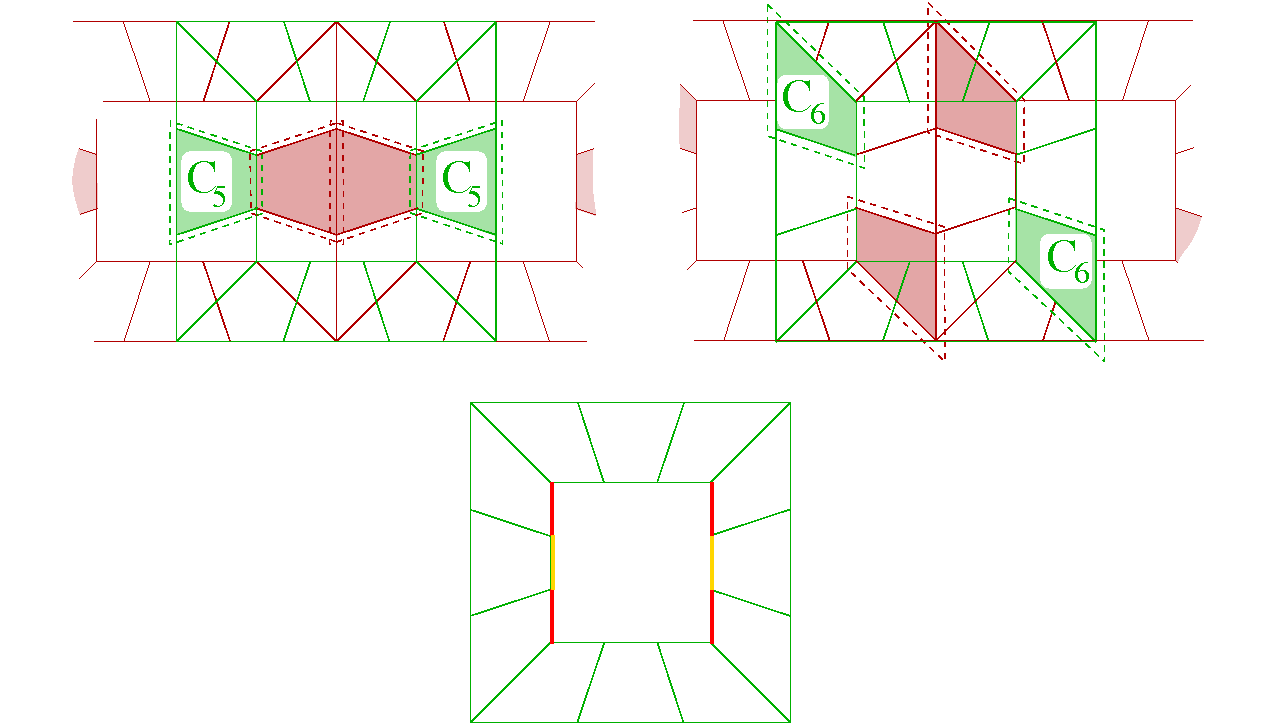
\includegraphics[width=\textwidth]{fig_overlap.png}\hspace*{-2mm}
%\end{minipage}
\begin{minipage}{.3\textwidth}
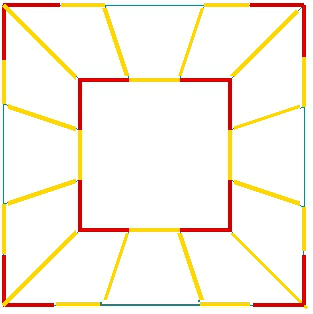
\includegraphics[width=\textwidth]{bdyclass.jpg}
\end{minipage}
%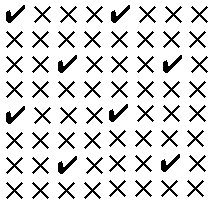
\includegraphics[width=.2\textwidth]{fig/sublattice-2.jpg}
\caption[caption]{
%\textcolor{red}{
%{\it Left top}: the supports of $m_j$ (green) and $m_j(\cdot+\V{\pi}_2$ (red) for $j = 5,6$ after smoothing, overlap on the vertical boundary at $\omega_1 =  \pm \pi/2$ of $C_5$ (green) and its shift (red) by $\boldsymbol{\pi}_2 = (\pi,0)$. Note that two copies of shifted $S_0$ (red) overlap the un-shifted $S_0$(green) due to the $(2\pi,2\pi)$ periodicity of $m_j$. Only $m_0$ and $m_5$ have overlapping smoothed boundaries by $\boldsymbol{\pi}_2$. 
%\\\hspace{\textwidth}
%{\it Left bottom}: intersection of $\mathcal{B}(0,\boldsymbol{\pi}_2)$ and $\mathcal{B}(5,\boldsymbol{\pi}_2)$ in yellow and $\mathcal{C}(0,\boldsymbol{\pi}_2) = \mathcal{B}(0,\boldsymbol{\pi}_2)\setminus\mathcal{B}(5,\boldsymbol{\pi}_2)$ in red. Smoothing $m_0$ in the red (singular) region is impossible without violating \eqref{eq: shift-cancel}. %This leads to the distinction between regular (yellow) and singular (red) boundaries at $omega_1 = \pm\pi/2$.
%\\\hspace{\textwidth}
%{\it Right}: 
Boundary classification, singular (red) and regular (yellow) }%after similar arguments for all shifts $\boldsymbol{\pi}_i$.}
 %}
\label{fig: boundary}
\end{figure}

\begin{comment}
%\subsection{Boundary classification}
 After smoothing the $m_j$'s, the shift cancellation \eqref{eq: shift-cancel} may fail to hold as $supp(m_j)$ and $(supp(m_j)-\boldsymbol{\pi})$ may overlap near the smoothed boundaries, see Fig. \ref{fig: boundary}, illustrating $m_5(\boldsymbol{\omega})\overline{m_5(\boldsymbol{\omega} + \boldsymbol{\pi}_2)}\not\equiv 0.$
For simplicity, we introduce the following notations: let 
$\mathcal{B}(j,\boldsymbol{\pi}) =  supp(m_j)\cap\,(supp(m_j)-\boldsymbol{\pi})$ be the support of  $m_j(\boldsymbol{\omega})\overline{m_j(\boldsymbol{\omega} + \boldsymbol{\pi})}$ associated to $m_j$ and shift $\boldsymbol{\pi}$;
let $\mathcal{C}(j,\boldsymbol{\pi}) = \mathcal{B}(j,\boldsymbol{\pi}) \setminus \bigcup_{j'\neq j}\mathcal{B}(j',\boldsymbol{\pi})$. 
%In addition, we may introduce the (slight abuse of) notation $C_0 = S_1$.
\begin{lem}\label{lem: singular-bdy}
Shift cancellation \eqref{eq: shift-cancel} can hold for shift $\boldsymbol{\pi}\in\Gamma_0\setminus\{\boldsymbol{0}\}$, only if $\mathcal{C}(j,\boldsymbol{\pi})=\varnothing,\, \forall\, 0\leq j\leq 6$; 
it can hold for shift $\boldsymbol{\pi}\in\Gamma_1\setminus\Gamma_0$, only if $\mathcal{C}(j,\boldsymbol{\pi})=\varnothing,\, \forall\, 1\leq j\leq 6$. 
\end{lem}
\noindent{\it Proof.} Observe that, on $\mathcal{C}(j,\boldsymbol{\pi})$, $m_j(\boldsymbol{\omega})\overline{m_{j}(\boldsymbol{\omega}+\boldsymbol{\pi})} \not\equiv 0$ but $m_{j'}(\boldsymbol{\omega})\overline{m_{j'}(\boldsymbol{\omega}+\boldsymbol{\pi})} \equiv 0,\, \forall j' \neq j$, hence \eqref{eq: shift-cancel} doesn't hold. $\hfill\square$
%Furthermore, the identity summation constraint \eqref{eq: id-sum} implies that $|M_j(\boldsymbol{omega})| = 1$ on $\mathcal{C}(j,\boldsymbol{\nu}),\,\forall\boldsymbol{\nu}$, hence the discontinuity of $M$-functions across these boundaries is unavoidable.
 
Therefore, boundaries that after smoothing make $\mathcal{C}(j,\boldsymbol{\pi})$ non-empty are called {\it singular}; the rest are {\it regular}. We next provide an explicit boundary classification method:
\begin{prop}\label{prop: class-bdy}
$\forall\, 1\leq j\leq 6$, let $supp(m_j) = \ov{$C_j$}$, then the boundary of $C_j$ is $\partial C_j=\bigcup_{i \neq 0}\mathcal{B}(j,\boldsymbol{\pi}_i)$. The set of singular boundaries of $\partial C_j$ is $\bigcup_{i\neq 0}\mathcal{C}(j,\boldsymbol{\pi}_i)$, whereas its compliment set is the regular boundary set.
 \end{prop}
\noindent{\it Proof.} Since $\bigcup_i(C_j+\boldsymbol{\pi}_i) = S_0$, $\partial C_j\subset \bigcup_{i\neq 0} (\ov{$C_j$}+\boldsymbol{\pi}_i) $. Therefore, $\partial C_j\subset\bigcup_{i\neq 0}\mathcal{B}(j,\boldsymbol{\pi}_i)$. On the other hand, $\mathcal{B}(j,\boldsymbol{\pi}_i)\subset \partial\mathbf{C}_j, \forall \, i\neq 0$, hence the union of them is a subset of $\partial C_j$. It follows that $\mathcal{B}(j,\boldsymbol{\pi}_i)$ form a partition of the boundary $\partial C_j$. The partition of $\partial C_j$ into singular and regular boundaries follows from Lemma \ref{lem: singular-bdy}.$\hfill\square$

 The case of $\partial S_1$ is similar where $\mathcal{B}(0,\boldsymbol{\pi}),\,\boldsymbol{\pi}\in\Gamma_0\setminus\{0\}$ are considered. We use the notation $\mathcal{B}_s(j,\boldsymbol{\pi}),\mathcal{C}_s(j,\boldsymbol{\pi})$ for the special case $supp(m_j) = \ov{$C_j$}$ hereafter.
The boundary classification based on Proposition \ref{prop: class-bdy} is shown in the right of Fig. \ref{fig: boundary}, where the boundaries on the four corners of both $S_0$ and $S_1$ are singular: smoothing is then not allowed there.

\begin{prop}\label{prop: jump}
Let $\mathcal{C} = \mathcal{C}_s(j_1,\boldsymbol{\pi}_{i_1})\cap \mathcal{C}_s(j_2,\boldsymbol{\pi}_{i_2})$, if $m_{j_1}, m_{j_2}$ satisfy \eqref{eq: id-sum}, \eqref{eq: shift-cancel}, then $|m_{j_1}|=\mathbbm{1}_{\mathbf{C}_{j_1}},\,|m_{j_2}|=\mathbbm{1}_{\mathbf{C}_{j_2}}$ on $\mathcal{C}$.
\end{prop}
\noindent{\it Proof.} Suppose the common singular boundary $\mathcal{C}$ is non-empty and observe that $\mathcal{C}\subset(C_{j_1})\cap(C_{j_2})$. Since $m_{j_1}$ cannot be smoothed on $\mathcal{C}_s(j_1,\boldsymbol{\pi}_{i_1})$, $|m_{j_1}| = 0$ on $\mathcal{C}_s(j_1,\boldsymbol{\pi}_{i_1})\setminus\mathbf{C}_{j_1}$, 
%Because $\mathcal{C}\subset\mathcal{C}_s(j_1,\boldsymbol{\nu}_1)\cap\partial\mathbf{C}_{j_2}$, 
and \eqref{eq: id-sum} implies that $|m_{j_2}| = 1$ there, or equivalently $|m_{j_2}|=\mathbbm{1}_{\mathbf{C}_{j_2}}$ on $\mathcal{C}$. Similarly, $|m_{j_1}|=\mathbbm{1}_{\mathbf{C}_{j_1}}$ on $\mathcal{C}.\hfill\square$

Prop. \ref{prop: jump} shows that if $m_j$ and $m_{j'}$ have common singular boundaries, then both will have a discontinuity across those boundaries. For example, $\mathcal{C}_s(0,(\pi,0))\cap\mathcal{C}_s(4,(\pi/2,\pi/2)) = (\pi/2,(\pi/6,\pi/2))$, hence $m_0$ and $m_4$ both are discontinuous at $(\pi/2,(\pi/6,\pi/2))$. All the singular boundaries related to \eqref{eq: MRA} are such "double" singular boundaries.

\subsection{Pairwise smoothing of regular boundary}
%Despite of the singular boundaries, better spatial localization can be achieved by carefully smoothing the regular boundaries. 
The regular boundaries of both $C_{j_1}$ and $C_{j_2}$ with adjacent supports consist of $\mathcal{B}_s(j_1,\boldsymbol{\pi})\cap\mathcal{B}_s(j_2,\boldsymbol{\pi})$, which we denote by the triple $(j_1,j_2,\boldsymbol{\pi})$. The following proposition shows that the regular boundaries $(j_1,j_2,\boldsymbol{\pi})$ can be paired according to shift pairs $(\boldsymbol{\pi},-\boldsymbol{\pi})$, and the boundaries must be smoothed pairwise within their $\epsilon-$neighborhood, $\mathcal{B}_{\epsilon}(j_1,j_2,\boldsymbol{\pi})$ and $\mathcal{B}_{\epsilon}(j_1,j_2,-\boldsymbol{\pi})$.

\begin{prop}\label{prop: pair-smooth}
Given $(j_1,j_2,\boldsymbol{\pi})\neq \varnothing$, %let $\boldsymbol{\nu}'= -\boldsymbol{\nu}\in \mathbb{R}^2/(\mathbb{Z}^2)^*$, 
then $(j_1,j_2,-\boldsymbol{\pi})\neq\varnothing$. In addition, let $\mathcal{B}=\mathcal{B}_{\epsilon}(j_1,j_2,\boldsymbol{\pi})\cup\mathcal{B}_{\epsilon}(j_1,j_2,-\boldsymbol{\pi})$. Then the identity summation and shift cancellation conditions hold if
\begin{itemize}
\item[{\it (i)}] $m_j = \mathbbm{1}_{C_j},\quad\text{on }S_0,\; j\neq j_1,j_2$
\item[{\it (ii)}] $m_{j_1} =\mathbbm{1}_{C_{j_1}},\, m_{j_2} =\mathbbm{1}_{C_{j_2}},\quad \text{on }\mathcal{B}^c$\\[.5em]
\hspace*{-2em} and on $\mathcal{B}$ the following hold%\vspace*{.1em}
\item[{\it(iii)}] $|m_{j_1}|^2 + |m_{j_2}|^2 = 1,$ %\hfill on $ \mathcal{B}_{\epsilon}(j_1,j_2,\nu)\cup\mathcal{B}_{\epsilon}(j_1,j_2,\nu')$
\item[{\it (iv)}] $\sum_{j_1,j_2} m_j(\cdot)\overline{m_j(\cdot+\widetilde{\boldsymbol{\pi}})} = 0,\, \widetilde{\boldsymbol{\pi}} = \pm\boldsymbol{\pi}$
%\hspace*{8em} on $\mathcal{B}_{\epsilon}(j_1,j_2,\nu)$ and $\mathcal{B}_{\epsilon}(j_1,j_2,\nu)-\nu$
%\item[{\it (v)}] $\sum_{j_1,j_2} M_j(\cdot)\overline{M_j(\cdot+\boldsymbol{\nu}')} = 0.$ 
%\hspace*{7em} on $\mathcal{B}_{\epsilon}(j_1,j_2,\boldsymbol{\nu}')$ and $\mathcal{B}_{\epsilon}(j_1,j_2,\nu')-\nu'$
\end{itemize}
\end{prop}
\noindent{\it Proof}.
 We first show that $(j_1,j_2,-\boldsymbol{\pi})\neq\varnothing.$ By definition, $\mathcal{B}_s(j_1,\boldsymbol{\pi}) = supp(m_{j_1})\cap (supp(m_{j_1})-\boldsymbol{\pi}) = \left((supp(m_{j_1})+\boldsymbol{\pi})\cap supp(m_{j_1})\right)-\boldsymbol{\pi} = \mathcal{B}_s(j_1,-\boldsymbol{\pi})-\boldsymbol{\pi}.$ Rewrite $(j_1,j_2,\boldsymbol{\pi})$ by $\mathcal{B}_s(j_1,-\boldsymbol{\pi})$ and $\mathcal{B}_s(j_2,-\boldsymbol{\pi})$, we have $(j_1,j_2,-\boldsymbol{\pi}) = (j_1,j_2,\boldsymbol{\pi})+\boldsymbol{\pi}$, hence it's non-empty.
 
Because $(j_1,j_2,\pm\boldsymbol{\pi})\subset (\partial C_{j_1} \bigcap \partial C_{j_2})$ and $(\bigcup_{j}C_j)=S_0$, $(\bigcup_{j\neq j_1,j_2}C_j)\cap \mathcal{B} = \varnothing.$ Therefore, smoothing of $m_{j_1}$ and $m_{j_2}$ in $\mathcal{B}$ doesn't impact the region where other $m_j$'s are supported.

We then show that the cancellation conditions \eqref{eq: shift-cancel} hold for all shifts. Condition (i) and (ii) imply that $\mathcal{B}(j,\widetilde{\boldsymbol{\pi}})= \varnothing,\,\forall j,\widetilde{\boldsymbol{\pi}}\neq \pm \boldsymbol{\pi}$, hence \eqref{eq: shift-cancel} hold for $\widetilde{\boldsymbol{\pi}}\neq \pm \boldsymbol{\pi}$. %For $\boldsymbol{\nu}$, 
(i) implies $\mathcal{B}(j,\widetilde{\boldsymbol{\pi}}) = \varnothing,\,\forall j\neq j_1,j_2$, so then \eqref{eq: shift-cancel} is equivalent to (iv). %Similarly, \eqref{eq: shift-cancel} is equivalent to (v) under (i).
The identity summation \eqref{eq: id-sum} holds due to (i), (ii) and (iii).$\hfill\square$.

By Prop. \ref{prop: pair-smooth} we can smooth some pairs of regular boundaries starting from the Shannon-type directional wavelets with the simplified conditions (iii), (iv) and (v); (i) and (ii) can be removed as long as the initial $m_j$ satisfy \eqref{eq: id-sum} and \eqref{eq: shift-cancel} and every $\boldsymbol{\omega}\in S_0$ is not covered by more than two $m$ functions. We can thus smooth regular boundaries pairwise, one by one.

The next proposition gives an explicit design of $(m_{j_1}, m_{j_2})$ satisfying the simplified conditions (iii),(iv) in Proposition \ref{prop: pair-smooth}. %as well as a necessary condition for any valid design.
\begin{prop}\label{prop: m-design}
Let $C\subset S_0$, given $m_{j_1},m_{j_2}\neq 0$ continuous on $ C\cup(C+\boldsymbol{\pi})$, satisfying the following conditions
\begin{itemize}
\item[(i)] $\sum_{j_1,j_2}m_{j}(\boldsymbol{\omega})\overline{m_{j}(\boldsymbol{\omega}+\boldsymbol{\pi})} = 0$ \hspace*{2em} on $C$
\item[(ii)] $\sum_{j_1,j_2}|m_{j}(\boldsymbol{\omega})|^2= 1 $ \hspace*{5em} on $C\cup (C+\boldsymbol{\pi})$
\item[(iii)] $m_{j_1}(\boldsymbol{\omega})m_{j_2}(\boldsymbol{\omega}) = 0$\hspace*{5em} on $\partial C$ ;
\end{itemize}
then
$\quad|m_{j_1}(\boldsymbol{\omega})| = |m_{j_2}(\boldsymbol{\omega}+\boldsymbol{\pi})|,\quad |m_{j_2}(\boldsymbol{\omega})| = |m_{j_1}(\boldsymbol{\omega}+\boldsymbol{\pi})|.$\\[1mm]
Furthermore, if $m_{j} = e^{i\boldsymbol{\omega}^{T}\boldsymbol{\eta}_{j}}\mathrm{m}_{j},\quad j=j_1,j_2, \text{ on }C,$ where $\mathrm{m}_j$ is a real-valued function, % $\mathcal{M}_{j_1}$ and $\mathcal{M}_{j_2}$,  phase $\eta_1,\eta_2$ s.t.
$e^{i\boldsymbol{\pi}^T(\boldsymbol{\eta}_{j1}-\boldsymbol{\eta}_{j2})} = -1,$ and 
\[\mathrm{m}_{j_1}(\boldsymbol{\omega}) = \mathrm{m}_{j_2}(\boldsymbol{\omega}-\boldsymbol{\pi}),\;\mathrm{m}_{j_2}(\boldsymbol{\omega}) = \mathrm{m}_{j_1}(\boldsymbol{\omega}-\boldsymbol{\pi}),\text{ on }C+\boldsymbol{\pi},\] 
%where $\mathcal{M}_{j1},\,\mathcal{M}_{j2}$ are 
then $(i)$ holds.
\end{prop}
\noindent{\it Proof.} 
To prove the necessary condition, note that (i) implies $|m_{j_1}(\boldsymbol{\omega})|^2|m_{j_1}(\boldsymbol{\omega+\pi})|^2 = |m_{j_2}(\boldsymbol{\omega})|^2|m_{j_2}(\boldsymbol{\omega+\pi})|^2$; the condition then follows from (ii).
For the sufficient construction, check by directly substituting the construction into (i). $\hfill\square$
%For the necessary condition, we prove in two cases. Suppose $|M_{j_1}|  = |M_{j_2}|$ on $\omega$, then (ii) implies $|M_{j_1}| = |M_{j_2}| = \frac{1}{2}$ on $\omega$. From (i), it's necessary $|M_{j_1}(\boldsymbol{omega}+\boldsymbol{\nu})|=|M_{j_2}(\boldsymbol{omega}+\boldsymbol{\nu})|$ on $\omega$, or equivalently, $|M_{j_1}| = |M_{j_2}|$ on $\omega + \boldsymbol{\nu}$. Apply (ii) again, we have $|M_{j_1}| = |M_{j_2}| = \frac{1}{2}$ on $\omega+\boldsymbol{\nu}$, therefore, $|M_{j_1}(\boldsymbol{omega})| = |M_{j_2}(\boldsymbol{omega}+\boldsymbol{\nu})|=|M_{j_2}(\boldsymbol{omega})| = |M_{j_1}(\boldsymbol{omega}+\boldsymbol{\nu})|=\frac{1}{2}.$%However, (iii) implies that either $M_{j_1}$ or $M_{j_2}$ decays to zero on the boundary, therefore, $|M_{j_1}$ and $|M_{j_2}|$ cannot be constant.

%Suppose now $|M_{j_1}(\boldsymbol{omega})| = |M_{j_2}(\boldsymbol{omega}+\boldsymbol{\nu})|$ on $\omega$, then (i) implies $|M_{j_2}(\boldsymbol{omega})| = |M_{j_1}(\boldsymbol{omega}+\boldsymbol{\nu})|$ on $\omega$.


Proposition \ref{prop: m-design} breaks down the design of $(m_{j_1},m_{j_2})$ into a pair of real functions $(\mathrm{m}_{j_1}, \mathrm{m}_{j_2})$ on $\mathcal{B}_{\epsilon}(j_1,j_2,\boldsymbol{\pi})$ and two vectors $\boldsymbol{\eta}_1,\boldsymbol{\eta}_2$; then $(\mathrm{m}_{j_1}, \mathrm{m}_{j_2})$ on $\mathcal{B}_{\epsilon}(j_1,j_2,-\boldsymbol{\pi})$ are automatically determined. %When all regular boundaries adopt this smoothing scheme,  each $\mathcal{M}_j$ has to locally match up with every $\mathcal{M}_{j'}$'s that shares a regular boundary $(j,j',\nu)$. Therefore, we may focus on 
The only constraint on $(\mathrm{m}_{j_1},\mathrm{m}_{j_2})$ for (ii) in Proposition \ref{prop: m-design} to hold is that on $\mathcal{B}_{\epsilon}(j_1,j_2,\boldsymbol{\pi})$, $\sum_{j_1,j_2}|\mathrm{m}_{j}(\boldsymbol{\omega})|^2= 1$, which is easy to be satisfied.
We may construct all local pairs of $(\mathrm{m}_{j_1},\mathrm{m}_{j_2})$ separately, and put together afterwards different pieces of each $\mathrm{m}_j$ located in different regular boundary neighborhoods $\mathcal{B}_{\epsilon}(j,j',\boldsymbol{\pi})$. 

\vspace*{.2em}
%The phase term $e^{i\boldsymbol{omega}^T\boldsymbol{\eta}_j}$ is preferably defined on the full frequency domain, hence $\boldsymbol{\eta}_j$'s need to be solved globally. This global phase problem is stated precisely in t
The next proposition gives % conditions for the $\boldsymbol{\eta}_j$ as well as 
one solution, easy to verify.
\begin{prop}\label{prop: phase}
Applying Proposition \ref{prop: m-design} to all regular boundaries requires a set of phases $\{\boldsymbol{\eta}_j\}_{j = 0}^6,$ s.t.\[\textstyle e^{i\boldsymbol{\nu}^T(\boldsymbol{\eta}_{j1}-\boldsymbol{\eta}_{j2})} = -1, \quad\forall (j_1,j_2,\boldsymbol{\pi})\in\Delta,\]
{\small\begin{multline*}
\Delta = \Bigl\{\big(0,2,(0,\pi)\big),\, \big(0,5,(\pi,0)\big),\,\big(1,3,(\pi,0)\big),\,\big(4,6,(0,\pi)\big),\\
\big(1,6,(\pi/2, 3\pi/2)\big),\,\big(2,3,(\pi/2, 3\pi/2)\big),\,\big(4,5,(\pi/2, 3\pi/2)\big), \\
\big(3,4,(\pi/2, \pi/2)\big),\big(1,2,(\pi/2, \pi/2)\big),\,\big(5,6,(\pi/2, \pi/2)\big)\Bigr\}
\end{multline*}}
The following is a (non-unique) solution: 
{\small\begin{multline*}\boldsymbol{\eta}_0 = (0,0),\,\boldsymbol{\eta}_1 = (0,0),\,\boldsymbol{\eta}_2 = (1,1),\,\boldsymbol{\eta}_3 = (1,-1),\\
\boldsymbol{\eta}_4 = (0,2),\,\boldsymbol{\eta}_5=(1,1),\,\boldsymbol{\eta}_6 = (-1,1).
\end{multline*}}
\end{prop}

To summarize, Proposition \ref{prop: m-design} and \ref{prop: phase} introduce the following regular boundary smoothing scheme for the $m$ functions:
\begin{description}% prevent items from splitting
\item[construction of orthonormal basis]\
\begin{itemize}
\item[1.] First, set $\mathrm{m}_j = \mathbbm{1}_{C_j}$; then smoothen these across a pair of regular boundaries $(j_1,j_2,\pm\boldsymbol{\pi})$ following steps 2, 3.
\item[2.]  On $\mathcal{B}_{\epsilon}(j_1,j_2,\boldsymbol{\pi})$,\\
\hspace*{2em} design $(\mathrm{m}_{j_1},\mathrm{m}_{j_2}),\quad$ s.t.
$\sum_{j_1,j_2}|\mathrm{m}_{j}(\boldsymbol{\omega})|^2= 1$.
\item[3.] On $\mathcal{B}_{\epsilon}(j_1,j_2,-\boldsymbol{\pi})$, \\
\hspace*{2em}let $\mathrm{m}_{j_1}(\boldsymbol{\omega}) = \mathrm{m}_{j_2}(\boldsymbol{\omega}-\boldsymbol{\pi})$, $\mathrm{m}_{j_2}(\boldsymbol{\omega}) = \mathrm{m}_{j_1}(\boldsymbol{\omega}-\boldsymbol{\pi})$\vspace*{.1em}
\item[4.] Repeat step 2 and 3 for all $(j_1,j_2,\boldsymbol{\pi})\in\Delta$. 
\item[5.]$m_j(\boldsymbol{\omega}) =e^{i\boldsymbol{\omega}^T\boldsymbol{\eta}_j} \mathrm{m}_j(\boldsymbol{\omega}),$ on $S_0$, with the $\boldsymbol{\eta}_j$ of Prop. \ref{prop: phase}.
\end{itemize}
\end{description}

\begin{figure}[!t]
\centering
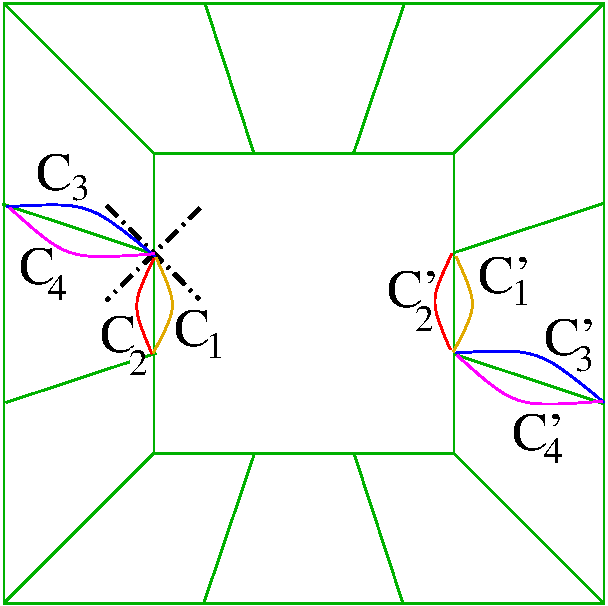
\includegraphics[height=.3\textwidth]{contour_design.pdf}\hspace*{2mm}
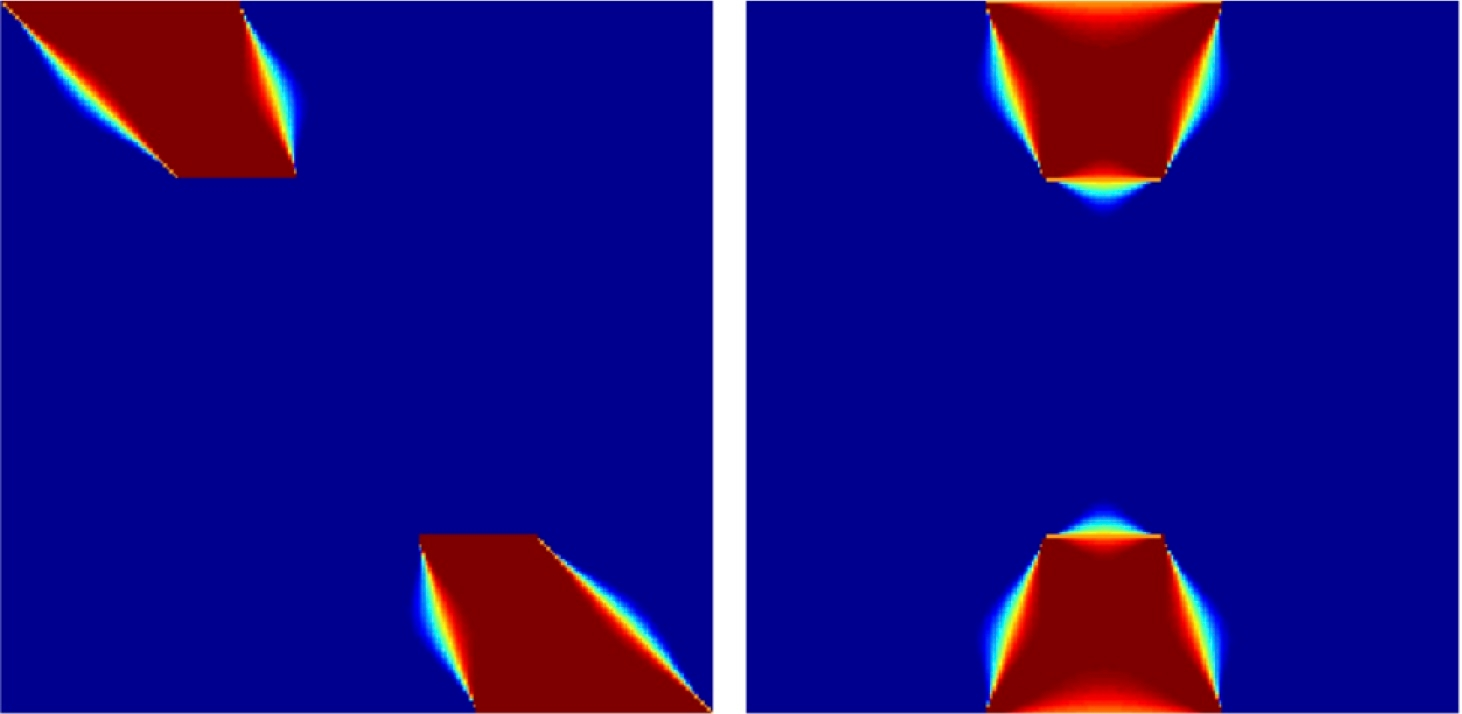
\includegraphics[height=.3\textwidth]{smsh-sh.jpg}
\caption{ Left: contour design of $supp(m_5)$, Right: frequency support $|\hat{\psi}^j|$}
\label{fig: design}
\end{figure}

%\section{Quasi-shearlet bases construction}\label{sec: bases construction}
%In this section, we present a family of quasi-shearlet bases constructed based on the $M$-function design discussed in section \ref{sec: design} using our proposed MRA framework.

We apply this to smooth all the regular boundaries except those on the boundary of $S_0$. Near a regular boundary $\mathcal{B}_{\epsilon}(j,j',\boldsymbol{\pi})$, the discontinuity of $|m_j|$ from 0 to 1 depends on $\mathrm{m}_j$; the contour of stop-band(pass-band) is the boundary of level set $\{\mathrm{m}_j(\boldsymbol{\omega}) = 0\}\,(\{\mathrm{m}_j(\boldsymbol{\omega}) = 1\}$). Fig. \ref{fig: design} shows our design of the stop-band/pass-band contours of regular boundaries {\small $\big(5,6,(\frac{\pi}{2},\frac{\pi}{2})\big)$} and {\small $\big(0,5,(\pi,0)\big)$}. The contours intersect only at the vertices of $C_5$, e.g. $supp(m_5)\cap supp(m_6)\cap supp(m_0)$ contains just one point. % as the relaxed condition (1) in Proposition \ref{prop: pair-smooth}. 
Moreover, we set $\mathrm{m}_5$ to be symmetric with respect to the origin near both regular boundaries. 

The contours related to other regular boundaries are designed likewise to achieve the best symmetry; the corresponding wavelets are real. Fig.\ref{fig: design} (right) shows the frequency support of directional wavelets generated by such design; Fig.\ref{fig: many-squares}(a) shows the wavelets and scaling function in space domain. One easily checks (using Theorem \ref{thm: basis cond}) that this is an orthonormal basis.

\begin{figure}[!t]
\centering
\hspace*{-5mm}\vspace*{-2mm}
\begin{minipage}[t]{\textwidth}
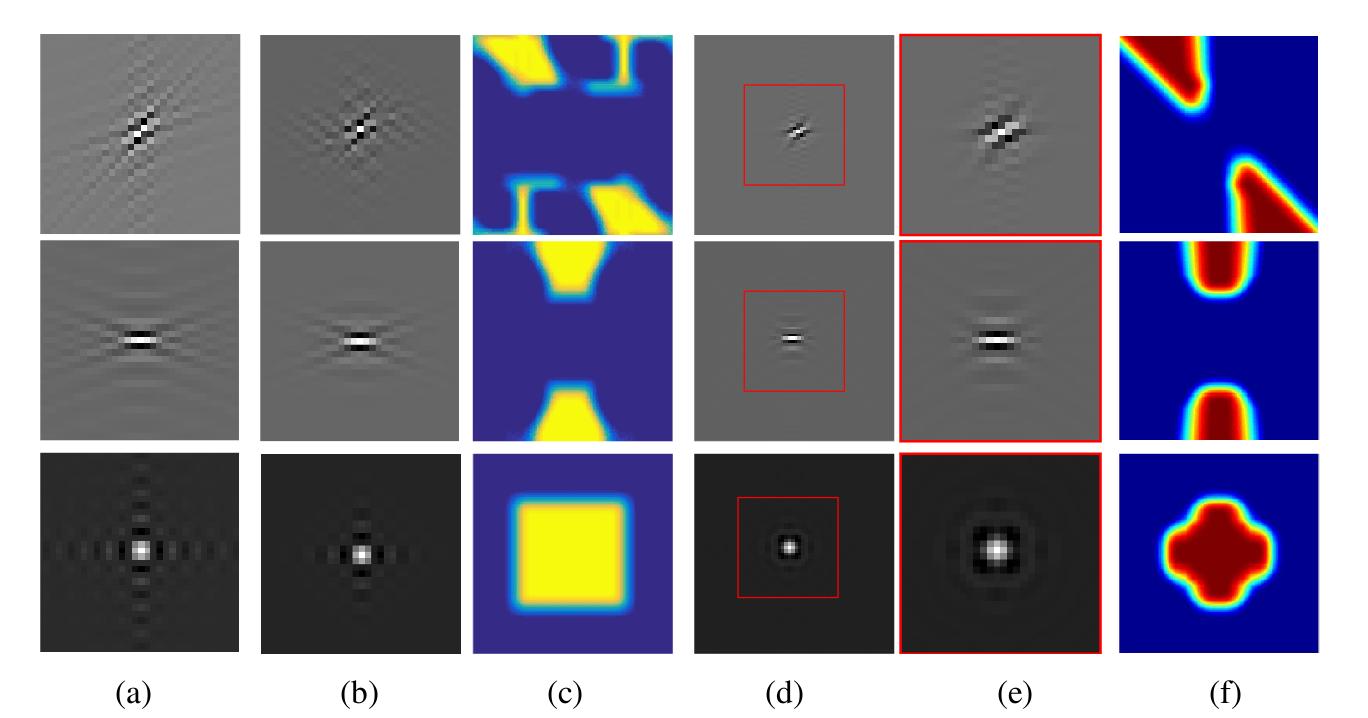
\includegraphics[width=\textwidth]{many_squares_new.png}
\end{minipage}\hspace*{1mm}
\caption{ directional wavelets $\psi^1$, $\psi^2$ and scaling function $\phi$ in different constructions (a) our directional wavelet orthonormal basis, whose frequency support is shown in Fig. \ref{fig: design};(b) Durand's directional wavelet; (c) $m-$ functions of wavelets in (b). (d) our directional wavelet frame; (e) zoom in on (d); (f) $m-$ functions of wavelets in (d);  Our basis construction in (a) has good frequency localization, but slowly decaying spatial oscillation; Durand's construction in (b) has good spatial localization but non-localized frequency support; our frame construction in (d) has both good frequency localization and spatial localization. Note that plots (a),(b),(e) are at the same resolution.}
\label{fig: many-squares}
\vspace*{-3mm}
\end{figure}

Although the wavelets orient in six directions, they are not very well localized spatially, due to the singular boundaries on the corners of the low-frequency square $S_1$, where the discontinuity in the frequency domain is inevitable. The lack of smoothness at the vertices of $m_2$ and $m_5$ could possibly be avoided by using a more delicate (but more complicated) design around the vertices $(\pm\frac{\pi}{2},\pm\frac{\pi}{6})$ allowing triple overlapping of $m-$functions.% yet Proposition \ref{prop: pair-smooth} and consequently Proposition \ref{prop: M-design} are nolonger helpful.

Allowing a bit of redundancy (abandoning critical downsampling), we show next how to construct a frame with low redundancy that has much better spatial localization.
\end{comment}